\section{Auswertung}
\label{sec:Auswertung}
\subsection{Verwertung der Messwerte zur zeitabhängigkeit der Amplitude}
\label{subsec:AuswertungA}
\subsubsection{Berechnung des effektiven Dämpfungswiderstandes}
\label{subsubsec:Erste Rechnung}
Um den effektiven Dämpfungswiderstand zu bestimmen kann man folgende Formel betrachten: 
\begin{equation}
  \label{eqn:Abklingdauer}
  \frac{1}{2\pi\mu} = \frac{2L}{R_{eff}}
\end{equation}
Durch Umstellen auf $R_{eff}$ ergibt sich eine Berechnungsformel:
\begin{equation}
  \label{Abklingdauer1}
  \Longleftrightarrow R_{eff} = 4\pi\mu L
\end{equation}
Um nun $R_{eff}$ zu berechnen wird zunächst eine Fit-Kurve durch die Messwerte gelegt (siehe \autoref{fig:PlotZuA}).
\begin{figure}
  \centering
  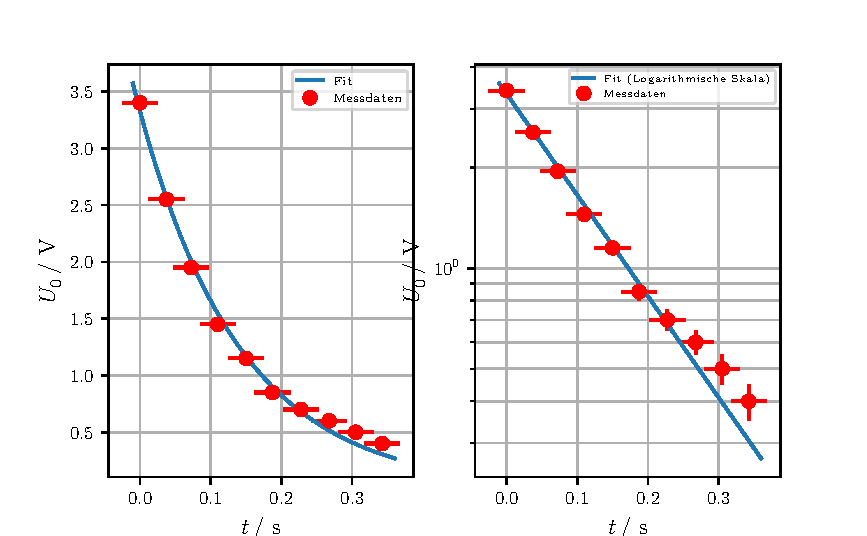
\includegraphics[width=0.7\textwidth]{PlotZuA.pdf}
  \caption{Darstellung der Messwerte zur ersten Messaufgabe}
  \label{fig:PlotZuA}
\end{figure}
Man benötigt nun noch den Faktor $2\pi\mu$. Diesen kann man durch die erstellte exponentielle Regression 
bestimmen, da $2\pi\mu$ dem positiven Faktor des Exponenten der erstellten Exponentialfunktion entspricht. 
Daher ist $2\pi\mu = 6.98[\mu]$, wobei $[\mu]$ der Einheit von $\mu$ entspricht. 
$R_{eff}$ ergibt sich durch einsetzen zu:
\begin{equation}
  R_{eff} = (2\cdot 6.98\cdot \num{16.87\pm 0.05}) \unit{\ohm} = (\num{117.75 \pm 0.05})\,\unit{\ohm}
\end{equation}